\section{Dynamic Mode Decomposition (DMD)}
Let us go back to the case of a linear dynamical system
\begin{equation*}
    \vb{x}_{n+1} = \vb*{A}\vb{x}_n, \qquad \vb*{A}\in\R^{n\times n}.
\end{equation*}
As already discussed, in order to extract the dynamic characteristics we need to analyze the spectral properties of $\vb{A}$. However, in a data-drive perspective, we cannot assume that we have access to $\vb*{A}$, but only to a sequence of snapshots. Therefore, we are interested in computing the eigenpairs of $\vb{A}$, or at least the dominant ones, from a sequence of snapshots
\begin{equation*}
    \label{krylov_space}
    \vb*{V}_1^N = \left[\vb{v}_1, \vb{v}_2, \dots, \vb{v}_N\right] = \left[\vb{v}_1, \vb*{A}\vb{v}_1, \dots, \vb*{A}^N\vb{v}_1\right].
\end{equation*}
Since the columns of $\vb*{V}_1^N$ span a Krylov subspace, it is natural to apply a Krylov subspace method. As we do not have access to the matrix $\vb*{A}$ and we cannot compute products of vectors by this matrix, we cannot directly apply numerically stable algorithms such as the Arnoldi method, and we can rely only on the sequence of snapshots we are given in input. \emph{Dynamic Mode Decomposition} (DMD) \cite{schmid_dynamic_2010} is a variant of the Arnoldi method that does not require computing multiplications by $\vb*{A}$, nor any knowledge of the matrix. 

Let us first suppose that, after a certain number of iterates, we found an $\vb*{A}$-invariant Krylov subspace and that $\vb{v}_N$ can be expressed as a linear combination of the previous linearly independent snapshots, i.e.
\begin{equation}
    \label{vn_exact}
    \vb{v}_N = a_1 \vb{v}_1 + \dots + a_{N-1} \vb{v}_{N-1} = \vb{V}_1^{N-1}\vb{a}, \qquad \vb{a}\in\R^{N-1}.
\end{equation}
We can rewrite the relation in \eqref{vn_exact} as:
\begin{equation*}
    \vb*{A}\vb*{V}_1^{N-1} = \vb*{V}_2^{N} = \vb*{V}_1^{N-1}\vb*{S}
\end{equation*}
where $\vb*{S}$ is the companion matrix associated with $\vb{a}$, defined by:
\begin{equation}
    \label{S_definition}
    \vb*{S} :=
   \begin{bmatrix}
   0     &        &       &      & a_1 \\
   1     & 0      &       &      & a_2 \\
         & \ddots & \ddots&      & \vdots \\ 
         &        & 1     & 0    & a_{N-2} \\
         &        &       & 1    & a_{N-1} \\
   \end{bmatrix}.
\end{equation}
The eigenvalues of $\vb*{S}$ are also eigenvalues of $\vb*{A}$. Indeed, if $\vb*{S}\vb{x} = \lambda \vb{x}, \,\, \vb{x}\neq 0$ then $\vb{y} = \vb{V}_1^{N-1}\vb{x}\neq 0$ (we assumed that the first $N-1$ snapshots are linearly independent) and $\vb*{A}\vb{y} = \vb*{A}\vb{V}_1^{N-1}\vb{x} = \vb{V}_1^{N-1}\vb*{S}\vb{x} = \lambda \vb{V}_1^{N-1}\vb{x} = \lambda \vb{y}$.

In general, $\vb{v}_N$ does not necessarily belong to the Span of the columns of $\vb*{V}_1^N$. However, as $N$ increases the snapshots tend to lie in the same direction (or at least in the same subspace) and we can expect that after a critical number of snapshots $\vb{v}_N$ \emph{almost} lies in the $\Span{(\vb*{V}_1^{N-1})}$, where by \emph{almost} we mean that the normalized difference between $\vb{v}_N$ and its projection onto $\Span{(\vb*{V}_1^{N-1})}$ is small. Therefore, again assuming that the previous vectors are linearly independent, we we want to write
\begin{equation}
    \label{vn_error}
    \begin{split}
        & \vb{v}_N = a_1 \vb{v}_1 + \dots + a_{N-1} \vb{v}_{N-1} + \vb{r}, \qquad \text{i.e.}\\
        & \vb*{A}\vb*{V}_1^{N-1}  = \vb*{V}_1^{N-1}\vb*{S} + \vb{r}\vb{e}_{N-1}^T
    \end{split}
\end{equation}
so that we minimize the norm of the residual $\vb{r} = \vb{v}_N - \vb*{V}_1^{N-1}\vb{a}$. To solve the corresponding least square problem, we compute the thin QR-decomposition of $\vb*{V}_1^{N-1} = \vb*{Q}\vb*{R}$ and then we obtain
\begin{equation}
    \label{a_qrleastsquare}
    \vb{a} = \vb*{R}^{-1} \vb*{Q}^*\vb{v}_N.
\end{equation}
The eigenvalues $\{\lambda_j\}_{j = 1}^{N-1}$ of the companion matrix $\vb*{S}$ are now approximations of the eigenvalues of $\vb*{A}$ and are called \emph{Ritz values}. The corresponding approximate eigenvectors $\vb{y}_j = \vb*{V}_1^{N-1}\vb{x}_j$, where $\vb{x}_j$ is an eigenvector of $\vb*{S}$ are the so called \emph{Ritz vectors}.

The above mentioned method was the original version of the DMD \cite{schmid_dynamic_2010}. However, even if it mathematically correct and equivalent to the Arnoldi method in exact arithmetic (see \Cref{section_dmd_arnoldi}), an implementation using the companion matrix $\vb*{S}$ gives rise to a numerically unstable algorithm that is usually not capable to extract more than one or two dominant eigenpairs. Using the Singular Value Decomposition (SVD) it is possible to obtain a mathematically equivalent but better-conditioned algorithm, which might be particularly useful when $\vb*{V}_1^{N-1}$ is close to singular (it is very likely to happen for large $N$). This second version of the DMD is what nowadays is referred as DMD. Suppose that we computed a SVD of the snapshots matrix
\begin{equation*}
    \vb*{V}_1^{N-1} = \vb*{U}\vb*{\Sigma}\vb*{W}^* \qquad \vb*{\Sigma}\in\R^{N-1\times N-1},
\end{equation*}
we can now rewrite \eqref{vn_error} as
\begin{equation}
    \label{vn_error_rewritten}
    \vb*{A}\vb*{U}\vb*{\Sigma}\vb*{W}^* = \vb*{U}\vb*{\Sigma}\vb*{W}^*\vb*{S} + \vb{r}\vb{e}_{N-1}^T = \vb*{V}_2^N
\end{equation}
and rearranging
\begin{equation}
    \label{S_tilde_definition}
    \vb*{U}^*\vb*{A}\vb*{U} = \vb*{U}^*\vb*{V}_2^N\vb*{W}\vb*{\Sigma}^{-1} =: \widetilde{\vb*{S}}.
\end{equation}
Once we have computed the eigenpairs $\{(\lambda_j, \vb{x}_j)\}_j$ of the matrix $\widetilde{\vb*{S}}$, which in this case is a full matrix and not of companion type, we obtain the Ritz values and vectors as $\{(\lambda_j, \vb*{U}\vb{x}_j)\}_j$. 

Besides the better conditioning, a great advantage of the SVD-based approach over the Arnoldi-based one is the opportunity to account for rank deficiency in $\vb*{V}_1^{N-1}$ and noise in the data by truncating the SVD of $\vb*{V}_1^{N-1}$. As observed in \cite{schmid_dynamic_2010}, without the use of TSVD it can be difficult to extract more than the first one or two dominant dynamic modes when using data from experiments, as the problem is ill-conditioned. 

As previously mentioned, the two approaches are equivalent since $\vb*{S}$ and $\widetilde{\vb*{S}}$ are linked through a similarity transformation. The residual of the least squares solution is orthogonal to the columns of $\vb*{U}$, hence from \eqref{vn_error_rewritten} and \eqref{S_tilde_definition}:
\begin{equation*}
    \begin{split}
    \widetilde{\vb*{S}} & =
    \vb*{U}^*\vb*{V}_2^N\vb*{W}\vb*{\Sigma}^{-1} =
    \vb*{U}^*(\vb*{U}\vb*{\Sigma}\vb*{W}^*\vb*{S} + \vb{r}\vb{e}_{N-1}^T)\vb*{W}\vb*{\Sigma}^{-1} = \\
    & = (\vb*{\Sigma}\vb*{W}^*) \vb*{S} (\vb*{W}\vb*{\Sigma}^{-1}) =
    (\vb*{\Sigma}\vb*{W}^*) \vb*{S} (\vb*{\Sigma}\vb*{W}^*)^{-1}    
    \end{split}
\end{equation*}

The SVD-based version of DMD is summarized in \Cref{alg_dmd}.

\begin{algorithm}
\caption{\textbf{: SVD-based DMD}}
\label{alg_dmd}
\textbf{Input:} $\vb{v}_1,\dots, \vb{v}_N$
\begin{algorithmic}[1]
\State Define the matrices $\vb*{V}_1^{N-1} = \left[\vb{v}_1,\dots,\vb{v}_{N-1}\right]$ and $\vb*{V}_2^{N} = \left[\vb{v}_2,\dots,\vb{v}_{N}\right]$.
\State Compute the (eventually truncated) SVD of $\vb*{V}_1^{N-1} = \vb*{U}\vb*{\Sigma}\vb*{W}^*,\,\, \vb*{\Sigma}\in\R^{p\times p}$.
\State Define the matrix $\widetilde{\vb*{S}} := \vb*{U}^*\vb*{V}_2^N\vb*{W}\vb*{\Sigma}^{-1}$.
\State Compute the eigenpairs $\{(\lambda_j, \vb{x}_j)\}_j$ of $\widetilde{\vb*{S}}$.
\State Compute the Ritz vector corresponding to the Ritz value $\lambda_j$ as $\vb{y}_j = \vb*{U}\vb{x}_j$. 
\end{algorithmic}
\textbf{Output:} Ritz values $\lambda_1,\dots,\lambda_{p}$ and corresponding Ritz vectors $\vb{y}_1,\dots, \vb{y}_p$
\end{algorithm}


\subsection{DMD and the Arnoldi method}
\label{section_dmd_arnoldi}
The Arnoldi method and the DMD are equivalent in exact arithmetic. In the following section, we will discuss and prove this statement, emphasizing why the Arnoldi algorithm is generally more stable.

The Arnoldi method computes an orthonormal basis of the Krylov subspace spanned by the columns of $\vb*{V}_1^{N-1}$ computing the snapshots implicitly. In particular, the algorithm computes a matrix $\vb*{Q}_{N-1} = \left[\vb{q}_1,\dots, \vb{q}_{N-1}\right]$ with columns that form an orthonormal basis of $\Span{(\vb*{V}_1^{N-1})}$ and: 
\begin{enumerate}[label=(\roman*)]
    \item $\vb*{V}_1^{N-1} = \vb*{Q}_{N-1} \vb*{R}_{N-1}$ is a thin QR-decomposition (with $\vb*{R}_{N-1}$ that is computed implicitly);
    \item $\vb*{H}_{N-1} = \vb*{Q}_{N-1}^* \vb*{A} \vb*{Q}_{N-1}$ is a Hessenberg matrix.
\end{enumerate}
Then the eigenpairs approximations are obtained from the eigenpairs of $\vb*{H}_{N-1}$.

This is mathematically equivalent to the DMD algorithm. Indeed from \eqref{vn_error} and \eqref{a_qrleastsquare} the residual $\vb{r}$ can be written as
\begin{equation*}
    \vb{r} = \vb{v}_N - \vb*{V}_1^{N-1}\vb*{R}_{N-1}^{-1}\vb*{Q}_{N-1}^*\vb{v}_N = v_N - \vb*{Q}_{N-1}\vb*{Q}_{N-1}^*\vb{v}_N
\end{equation*}
and therefore $\vb*{Q}_{N-1}^*\vb{r} = 0$. Finally plugging the QR-decomposition into \eqref{vn_error}
\begin{equation*}
    \vb*{A}\vb*{Q}_{N-1}\vb*{R}_{N-1} = \vb*{Q}_{N-1}\vb*{R}_{N-1}\vb*{S} + \vb{r}\vb{e}_{N-1}^T
\end{equation*}
and multiplying by $\vb*{Q}_{N-1}^*$ on the left and by $\vb*{R}_{N-1}^{-1}$ on the right
\begin{equation}
    \label{similarity_arnoldi_dmd}
    \vb*{H}_{N-1} = \vb*{Q}_{N-1}\vb*{A}\vb*{Q}_{N-1} = \vb*{R}_{N-1}\vb*{S}\vb*{R}_{N-1}^{-1}.
\end{equation}
Hence $\vb*{H}_{N-1}$ and $\vb*{S}$ are linked through a similarity transformation.

Although the two algorithms are equivalent mathematically and in exact arithmetic, the Arnoldi algorithm is numerically more stable. Indeed, as the number of snapshots increases, the vectors tend to become linearly dependent and therefore, the matrix $V_1^N$ becomes close to singular, hence ill-conditioned. Computing its QR-decomposition and $\vb{a} = \vb*{R}_{N-1}^{-1} \vb*{Q}_{N-1}^*\vb{v}_N$ might produce inaccurate results in floating-point arithmetic. Even if the previously mentioned problem can be partially solved using the SVD-based DMD and performing a truncated SVD, another major problem is intrinsic to the data-driven approach. One of the major strengths of the Arnoldi algorithm is that it does not even compute the vectors $\vb{x}_j = \vb*{A}^j \vb{x}_0$ because errors are already made in these computations. However, in a data-driven perspective, this is not possible since what we are given is a sequence of snapshots and not the matrix $\vb*{A}$. Hence, we trade-off better stability and convergence properties for an algorithm that only relies on $V_1^N$ and is therefore applicable to snapshots experimentally collected.

To compare numerically the algorithms, we performed 50 iterations with the matrix of size \texttt{n = 400} defined as \texttt{A = diag([5; randn(n-1,1)])} and random starting vector \texttt{x = rand(n,1)} normalized. \Cref{arnoldi_vs_DMD} shows the convergence of the approximations of the three dominant eigenvalues. It can be seen that the Arnoldi method is able to approximate all of them up to the epsilon-machine-precision, while both DMD algorithm fail in extracting the third dominant eigenvalue. Among the two versions of DMD, the SVD-based DMD shows better performances due to a better numerical stability.

\begin{figure}[h]
    \centering
    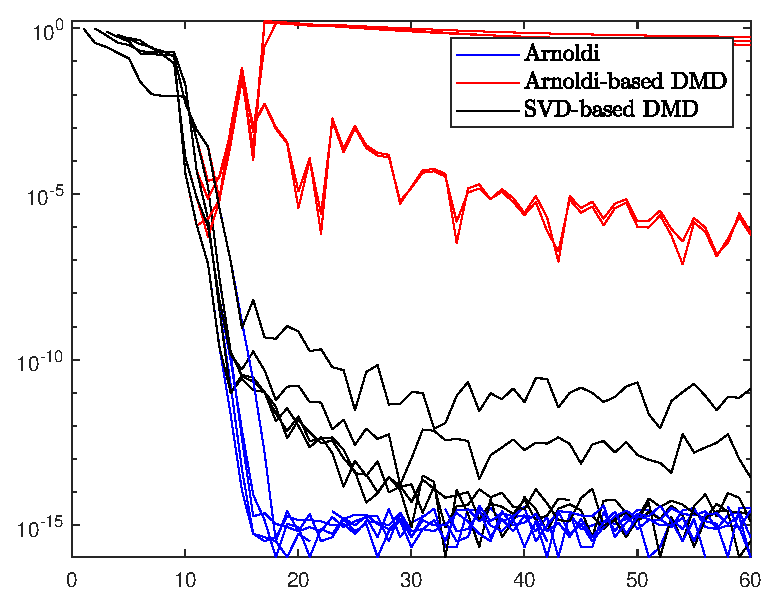
\includegraphics[width=0.5\linewidth]{../code/figures/Arnoldi_vs_DMD.eps}
    \caption{Convergence of the three dominant eigenvalues for the Arnoldi method and the two versions of the DMD algorithm.}
    \label{arnoldi_vs_DMD}
\end{figure}

\subsection{DMD for the Koopman Operator}
Suppose that instead of a snapshots along a single trajectory of snapshots $\vb{v}_1, \vb{v}_2, \dots, \vb{v}_N$ we are given snapshot pairs of the system state, $\{(\vb{x}_0^{(m)}, \vb{x}_1^{(m)})\}_{m = 1}^M$ with $\vb{x}_1^{(m)} = \vb{F}(\vb{x}_0^{(m)}) = \vb*{A}\vb{x}_0^{(m)}$. The first setting is just a particular case of the latter one, with $\vb{x}_0^{(m)} = \vb{v}_m,\,\,\vb{x}_1^{(m)} = \vb{v}_{m+1}$. However, even in the linear case, requiring in input only snapshot pairs instead of one trajectory allows us to explore as many different initial states as we want. This is of particular help if the trajectories tend to converge to an equilibrium. Let us define the data matrices
\begin{equation}
    \label{dmd_matrices}
    \vb*{X}_0 = \left[\vb{x}_0^{(1)}, \dots, \vb{x}_0^{(M)}\right] \qquad \vb*{X}_1 = \left[\vb{x}_1^{(1)}, \dots, \vb{x}_1^{(M)}\right]
\end{equation}
then it holds $\vb*{A}\vb*{X}_0 = \vb*{X}_1$. Then the least-squares solution is $\hat{\vb*{A}} = \vb*{X}_1\vb*{X}_0^{\dagger}$ and the eigenvalues of $\vb*{A}$ are approximated by the eigenvalues of $\hat{\vb*{A}}$. The DMD eigenvalues and modes are defined as the nonzero eigenvalues and corresponding eigenvectors of $\hat{\vb*{A}}$, respectively.

The version of the DMD algorithm presented above assumes that $\vb{x}_1^{(m)} = \vb{F}(\vb{x}_0^{(m)}) =  \vb*{A}\vb{x}_0^{(m)}$, i.e. that the system is linear. If the system is nonlinear, then $\hat{\vb*{A}}$ only provides the best-fit linear approximation of $\vb{F}$. However, even if the dynamics is nonlinear the Koopmam Operator is linear (and infinite dimensional). Therefore, we could apply the DMD algorithm to observables in order to obtain an approximation of the Koopman eigenvalues and modes. Let us consider a vector-valued observable $\vb{g} = \vb{g}(\vb{x})$ and its measurements over a set of arbitrary initial states $\{\vb{z}_1,\dots, \vb{z}_M\}$ and one step after. Let us define:
\begin{equation}
    \label{dmd_koopman_matrices}
    \begin{split}
        \vb*{G}_0 &= \left[\vb{g}(\vb{x}_1), \dots, \vb{g}(\vb{x}_M)\right] \\
        \vb*{G}_1 &= \left[\vb{g}(\vb{F}(\vb{x}_1)), \dots, \vb{g}(\vb{F}(\vb{x}_M))\right] = \left[\mathcal{K}\vb{g}(\vb{x}_1), \dots, \mathcal{K}\vb{g}(\vb{x}_M)\right].\\
    \end{split}
\end{equation}
In analogy to what has been done in the linear case, $\vb*{K} = \vb*{G}_1\vb*{G}_0^{\dagger}$ provides the best finite-dimensional approximation of the Koopman operator that can be achieved using the available data. Therefore, we can approximate the Koopman eigenvalues and modes from the eigendecomposition of $\vb*{K}$, as summarized in \Cref{alg_koopman_dmd}.

\begin{algorithm}[h]
\caption{\textbf{: DMD for Koopman Operator}}
\label{alg_koopman_dmd}
\textbf{Input:} Measurements of a vector values observable, collected in data matrices $\vb*{G}_0,\,\vb*{G}_1$ defined as in \eqref{dmd_koopman_matrices}.
\begin{algorithmic}[1]
\State Compute the (eventually truncated) SVD of $\vb*{G}_0 = \vb*{U}\vb*{\Sigma}\vb*{W}^*$.
\State Define the matrix $\vb*{K} := \vb*{U}^*\vb*{G}_1\vb*{W}\vb*{\Sigma}^{\dagger}$.
\State Compute the eigenpairs $\{(\lambda_j, \vb{x}_j)\}_j$ of $\vb*{K}$. Each nonzero eigenvalue is a DMD eigenvalue.
\State Compute the modes corresponding to the nonzero eigenvalue $\lambda_j$ as $\vb{v}_j = \vb*{U}\vb{x}_j$. 
\end{algorithmic}
\textbf{Output:} Approximation of the Koopman eigenvalues ($\lambda_j$) and modes ($\vb{v}_j$).
\end{algorithm}

It can be shown that also for nonlinear dynamics \Cref{alg_koopman_dmd} outputs, under fairly restrictive hypothesis, approximations of the Koopman modes and associated eigenvalues with respect to a chosen observable \cite{rowley_spectral_2009, tu_dynamic_2014}. However, as discussed in \cite{tu_dynamic_2014}, this method has limitations in the case of nonlinear dynamics and it is, therefore, a better choice to use methods such as Extended DMD \cite{williams_data-driven_2015} (see \Cref{section_edmd}).

\section{Extended Dynamic Mode Decomposition (EDMD)}
\label{section_edmd}
The \emph{Extended Dynamic Mode Decomposition} (EDMD), originally presented in \cite{williams_data-driven_2015}, is a method that seeks at approximating the Koopman Operator as a finite dimensional operator and then approximate the Koopman (eigenvalue, eigenfunction, mode) tuples from this finite dimensional approximation. The algorithm requires in input:
\begin{itemize}
    \item a dataset of snapshot pairs of the system state, $\{(\vb{x}_0^{(m)}, \vb{x}_1^{(m)})\}_{m = 1}^M$ with $\vb{x}_1^{(m)} = \vb{F}(\vb{x}_0^{(m)})$;
    \item a dictionary of observables $\mathcal{D} = \{\psi_1, \dots, \psi_K\} \subseteq \mathcal{D}(\mathcal{K})$. Let us define the vector-valued observable $\Psi:\Omega\to\C^{1\times k}$ as $\Psi(x) = [\psi_1(x), \dots, \psi_k(x)]$. The choice of the dictionary $\mathcal{D}$ is not easy and depends on the problem at hand. For the moment, let us assume that $\mathcal{D}$ is rich enough to approximate at least a few of the dominant Koopman eigenfunctions.
\end{itemize}

\subsection{Approximation of $\mathcal{K}$ and its eigenpairs}
Let $\phi\in\Span(\mathcal{D})$, then we can write:
\begin{equation*}
    \phi = \sum_{k=1}^K a_k\psi_k = \Psi\vb{a}, \qquad \vb{a}\in\C^K.
\end{equation*}
We aim at generating $\vb*{K}\in\C^{k\times k}$ finite dimensional approximation of $\mathcal{K}$ such that
\begin{equation}
    \label{k_finite_dimensional}
    \mathcal{K}\vb{\phi} = (\Psi \circ \vb{F})\vb{a} = \Psi\vb*K\vb{a} + r
\end{equation}
where the residual term $r = r(\vb{a}, \vb{x})$ is due to the fact that in general $\Span(\mathcal{D})$ is not $\mathcal{K}$-invariant. To obtain the "best" $\vb*{K}\in\C^{k\times k}$ it is natural to minimize the norm of the point-wise maximum of the residual of all possible $\phi\in\Span(\mathcal{D})$, i.e to solve the following problem \cite{colbrook_rigorous_2021}:
\begin{equation}
    \label{edmd_integral_problem}
    \argmin_{\vb*{K}\in\C^{K\times K}}\int_{\Omega} \max_{\vb{a}\in\C^k \\ \norm{\vb{a}} = 1}\abs{r(\vb{a}, \vb{x})}^2 d\omega(\vb{x}) = 
    \argmin_{\vb*{K}\in\C^{K\times K}}\int_{\Omega} \norm{\Psi(\vb{F}(\vb{x})) - \Psi(\vb{x})\vb*{K}}^2 d\omega(\vb{x}).
\end{equation}

We cannot directly compute the integral, thus we need to use a quadrature rule. We take as quadrature nodes our snapshot data $\{\vb{x}_0^{(m)}\}_{m = 1}^M$ with weights $\{w_m\}_{m = 1}^M$. The discretized problem reads:
\begin{equation}
\label{edmd_discretized_problem}
\begin{split}
    &\argmin_{\vb*{K}\in\C^{k\times k}} \sum_{j=1}^M w_j \norm{\Psi(\vb{F}(\vb{x}_0^{(j)})) - \Psi(\vb{x}_0^{(j)})\vb*{K}}^2 d\omega(\vb{x}) = \\
    = &\argmin_{\vb*{K}\in\C^{k\times k}} \sum_{j=1}^M w_j \norm{\Psi(\vb{x}_1^{(j)}) - \Psi(\vb{x}_0^{(j)})\vb*{K}}^2 d\omega(\vb{x}).
\end{split}    
\end{equation}
If we define the matrices
\begin{align}
\label{w_def}
\vb*{W} = \diag(w_1,\dots,w_M)\in\R_+^{M\times M} \\
\label{psi0_def}
\Psi_0 = \left[\Psi(\vb{x}_0^{(1)})^T,\dots,\Psi(\vb{x}_0^{(M)})^T\right]^T\in\C^{M\times K} \\
\label{psi1_def}
\Psi_1 = \left[\Psi(\vb{x}_1^{(1)})^T,\dots,\Psi(\vb{x}_1^{(M)})^T\right]^T\in\C^{M\times K}
\end{align}
we can write the weighted least-square problem in \eqref{edmd_discretized_problem} as 
\begin{equation}
    \label{edmd_discretized_problem_matrix}
    \argmin_{\vb*{K}\in\C^{k\times k}}\norm{\sqrt{\vb*{W}}(\Psi_1 - \Psi_0\vb*{K})}_F^2.
\end{equation}
Since this is a convex problem in $\vb*{K}$, it suffices to impose that the derivative (of the real and of the imaginary part) is zero, from which we get
\begin{equation}
    \label{discretized_problem_solution}
    (\Psi_0^*\vb*{W}\Psi_0)\vb*{K} = \Psi_0^*\vb*{W}\Psi_1 \,\,\Longrightarrow\,\, \vb*{K} = (\Psi_0^*\vb*{W}\Psi_0)^{\dagger}(\Psi_0^*\vb*{W}\Psi_1).
\end{equation}
If the weights are the same for all quadrature points, then from the properties of the Moore-Penrose inverse $\vb{K} = \Psi_0^{\dagger} \Psi_1$ and we are back to same matrix that we would obtain applying the DMD algorithm with vector-valued observable $\Psi$.

Observe that the involved matrice are
\begin{equation*}
    \label{psi_rewriting}
    \begin{split}
        \Psi_0^*\vb*{W}\Psi_0 & = \sum_{j=1}^M w_j \Psi(\vb{x}_0^{(j)})^* \Psi(\vb{x}_0^{(j)})\\
        \Psi_0^*\vb*{W}\Psi_1 & = \sum_{j=1}^M w_j \Psi(\vb{x}_0^{(j)})^* \Psi(\vb{x}_1^{(j)}).
    \end{split}
\end{equation*}
This rewriting is particularly advantageous when the number of snapshots is much larger than the size of the dictionary, i.e. $M >> K$, because each term of the sum can be computed individually and the products in \eqref{psi_rewriting} can be built iteratively, without the need of explicitly storing the matrices $\Psi_0,\,\Psi_1\in\C^{M\times K}$.

To approximate the eigenvalue-eigenfunction pair of the Koopman Operator, we use the eigenpairs of its finite dimensional approximation $\vb*{K}$. If $\lambda_j$ is an eigenvalue of $\vb*{K}$ with eigenvector $\bm{\xi}_j$, an approximation of an eigenvalue-eigenfunction pair of $\mathcal{K}$ is $(\lambda_j, \phi_j = \Psi\bm{\xi}_j)$.

A few final remarks for practical implementation of EDMD:
\begin{itemize}
    \item by reducing the size of the dictionary, we may assume without loss of generality that the matrix $(\Psi_0^*\vb*{W}\Psi_0)$ is non-singular. However, we might also consider using TSVD when computing its pseudo-inverse in practice.  
    \item Instead of computing the matrix $\vb*{K} = (\Psi_0^*\vb*{W}\Psi_0)^{\dagger}(\Psi_0^*\vb*{W}\Psi_1)$ and then its eigenpairs, it is often numerically more stable to solve the generalized eigenvalue problem $(\Psi_0^*\vb*{W}\Psi_0)\bm{\xi} = \lambda(\Psi_0^*\vb*{W}\Psi_1)\bm{\xi}$.
\end{itemize}

\subsection{Approximation of the Koopman modes for the full state observable}
Let us consider the full state observable
\begin{equation}
    \label{full_state_def}
    \vb{g}(\vb{x}) = 
    \begin{bmatrix}
    g_1(\vb{x}) \\
    \vdots \\
    g_d(\vb{x})
    \end{bmatrix} = 
    \begin{bmatrix}
    \vb{e}_1^*\vb{x} \\
    \vdots \\
    \vb{e}_d^*\vb{x}
    \end{bmatrix} = \vb{x}.
\end{equation}
Let us assume that $g_i\in\Span(\mathcal{D})$ for all $i = 1,\dots,d$. If this is not the case an intermediate step to project $g_i$ onto $\Span(\mathcal{D})$ is required, with the accuracy strongly depending on the choice of the dictionary. If $g_i\in\Span(\mathcal{D})$ we can write
\begin{equation}
    g_i = \sum_{k=1}^K b_{ki}\psi_k = \Psi\vb{b}_i
\end{equation}
and in matrix form
\begin{equation*}
    \vb{g} = \vb*{B}^T\Psi^T = (\Psi\vb*{B})^T, \qquad \vb*{B} = \left[\vb{b}_1, \dots,\vb{b}_d\right]\in\C^{k\times d}.
\end{equation*}
If we choose an orthonormal dictionary this step can be accomplished through the computation of the inner products $b_{ki} = \langle g_i, \psi_k \rangle$. This also accounts for the projection onto $\Span(\mathcal{D})$, if required.

Let $\bm{\Xi} = \left[\bm{\xi}_1,\dots,\bm{\xi}_K\right]$ be the matrix of the eigenvectors of $\vb*{K}$, the vector of approximate Koopman eigenfunctions $\Phi(\vb{x}) = \left[\phi_1(\vb{x}), \dots, \phi_K(\vb{x})\right]$ can be written as $\Phi = \Psi\bm{\Xi}$. Thus
\begin{equation}
    \vb{g} = \vb*{B}^T\Psi^T = \vb*{B}^T(\bm{\Xi}^T)^{-1}\Phi^T = (\bm{\Xi}^{-1}\vb*{B})^T\Phi^T.
\end{equation}
Since $\bm{\Xi}$ is the matrix of the eigenvectors of $\vb*{K}$, its inverse is $\bm{\Xi}^{-1} = \left[\vb{u}_1, \dots, \vb{u}_K\right]$ where $\vb{u}_i$ is the left eigenvector of $\vb*{K}$ also associated with $\lambda_i$ and appropriately scaled so that $\vb{u}_i^*\bm{\xi}_j = \delta_{ij}$. We can therefore compute the left eigenvectors of and letting  $\vb*{V} = (\vb*{U}^*\vb*{B})^T$, then
\begin{equation}
    \vb{g} = \vb*{V}\Psi^T = \sum_{k=1}^K \vb{v}_k\psi_k,
\end{equation}
i.e. $\vb{v}_j = (\vb{u}_j^*\vb*{B})^T$ is the $j$-th Koopman mode.

In conclusion, as summarized in \Cref{alg_edmd},  once we have computed the finite-dimensional approximation $\vb*{K}$ of the Koopman Operator:
\begin{itemize}
    \item the eigenvalues of $\vb*{K}$ are the EDMD approximation of the Koopman eigenvalues;
    \item the right eigenvectors of $\vb*{K}$ generate the approximation of the eigenfunctions;
    \item the left eigenvectors of $\vb*{K}$ generate the approximation of the Koopman modes.
\end{itemize}
If we are interested in an approximation of only a leading subset of eigenvalues, instead of a complete eigendecomposition of the matrix $\vb*{K}$ Krylov methods or other iterative methods might be considered to efficiently compute only the leading eigenpairs of $\vb*{K}$.

\begin{algorithm}
\caption{\textbf{: Extended Dynamic Mode Decomposition (EDMD)}}
\label{alg_edmd}
\textbf{Input}: Snapshot pairs of the system state, $\{(\vb{x}_0^{(m)}, \vb{x}_1^{(m)})\}_{m = 1}^M$, quadrature weights $\{w_m\}_{m = 1}^M$, dictionary of observables $\mathcal{D} = \{\psi_1, \dots, \psi_K\} \subseteq \mathcal{D}(\mathcal{K})$
\begin{algorithmic}[1]
\State Define the matrices $\vb*{W}$ \eqref{w_def}, $\Psi_0$ \eqref{psi0_def}, $\Psi_1$ \eqref{psi1_def}. 
\State Compute the matrices $(\Psi_0^*\vb*{W}\Psi_0)$ and $(\Psi_0^*\vb*{W}\Psi_1)$ .
\State Solve the generalized eigenvalue problem $(\Psi_0^*\vb*{W}\Psi_0)\bm{\xi} = \lambda(\Psi_0^*\vb*{W}\Psi_1)\bm{\xi}$.
\State Obtain the eigenfunctions as $\Phi = \Psi\bm{\Xi}$.
\If{want to compute eigenmodes}
    \State Write the (projection onto $\Span(\mathcal{D})$ of the) full observable $\vb{g}$ as $\vb{g} = \vb*{B}^T\Psi^T$.
    \State Compute the left eigenvectors $\vb{u}_j$ of $\vb*{K} = (\Psi_0^*\vb*{W}\Psi_0)^{\dagger}(\Psi_0^*\vb*{W}\Psi_1)$.
    \State Compute $\vb*{V} = (\vb*{U}^*\vb*{B})^T$, i.e $\vb{v}_j = (\vb{u}_j^*\vb*{B})^T$.
\EndIf
\end{algorithmic}
\textbf{Output:} Approximation of the Koopman eigenvalues ($\lambda_j$), eigenfunctions ($\phi_j$) and, eventually, eigemodes ($\vb{v}_j$).
\end{algorithm}


\section{Spectral pollution and Residual DMD (ResDMD)}
To compute the eigenvalues of the Koopman Operator, we approximate the infinite-dimensional operator $\mathcal{K}$ by a finite matrix. Therefore, even if some of the eigenvalues produced by the EDMD algorithm are reliable, most of them are not. \emph{Pseudospectra} \cite{trefethen_spectra_2005} are a tool that allow us to detect this so called \emph{spectral pollution} \cite{colbrook_rigorous_2021}, i.e. spurious eigenvalues of the matrix $\vb*{K}$ that are only due to the discretization and have no connection with the latent Koopman Operator. Given a matrix $\vb*{A}\in\C^{n\times n}$ and $\varepsilon > 0$, the $\varepsilon$-pseudospectrum o $\vb*{A}$ is defined as
\begin{equation}
    \label{pseudospectrum_matrix_def}
    \sigma_{\varepsilon}(\vb*{A}) = \left\{ \lambda\in\C \text{ : } \norm{(\vb*{A} - \lambda \vb*{I})^{-1}} > \frac{1}{\varepsilon}\right\} = \bigcup_{\norm{\vb*{B}} \leq \varepsilon} \sigma(\vb*{A}+ \vb*{B}),
\end{equation}
where $\sigma(\vb*{M})$ indicates the spectrum of the matrix $\vb*{M}$. However, $\mathcal{K}$ is an infinite dimensional operator and might be undounded, hence following \cite{trefethen_spectra_2005} we can define
\begin{equation}
    \label{pseudospectrum_koopman_def}
    \sigma_{\varepsilon}(\mathcal{K}) = \mathrm{cl}\left( \left\{ \lambda\in\C \text{ : } \norm{(\mathcal{K} - \lambda \cdot \mathrm{id})^{-1}} > \frac{1}{\varepsilon}\right\} \right) = \mathrm{cl}\left( \bigcup_{\norm{\vb*{B}} \leq \varepsilon} \sigma(\mathcal{K}+ \vb*{B}) \right)
\end{equation}
where $\mathrm{id}$ is the identity operator and $\mathrm{cl}$ is the closure of a set.

\subsection{ResDMD to remove spectral pollution}
The \emph{Residual DMD} (ResDMD) algorithm performs the same steps of EDMD, but then discards the approximate eigenpairs $\{(\lambda_j,\, \phi_j)\}_j$ that have a residual above a certain prescribed tolerance $\varepsilon$. Given a candidate eigenpair $(\lambda, \phi)$ of $\mathcal{K}$, where $\phi = \Psi\bm{\xi}$, to measure its accuracy we can consider the relative residual
\begin{equation}
    \label{residual_definiton}
    \begin{split}
        &\mathrm{res}(\lambda, \phi)^2 = \frac{\int_{\Omega} \abs{[\mathcal{K}\phi](x) - \lambda\phi(x)}^2\,\,d\omega(x)}{\int_{\Omega} \abs{\phi(x)}^2\,\,d\omega(x)} 
        = \frac{\langle (\mathcal{K} - \lambda \cdot\mathrm{id})\phi, (\mathcal{K} - \lambda \cdot \mathrm{id})\phi \rangle}{\langle\phi , \phi \rangle} = \\
        & = \frac{\sum_{j,k = 1}^K \overline{\xi}_j\xi_k \left( \langle\mathcal{K}\psi_k, \mathcal{K}\psi_j\rangle - \lambda \langle\psi_k, \mathcal{K}\psi_j\rangle - \overline{\lambda}\langle\mathcal{K}\psi_k, \psi_j\rangle + \abs{\lambda}^2 \langle\psi_k, \psi_j\rangle\right)}{\sum_{j,k = 1}^K \overline{\xi}_j\xi_k \langle\psi_k, \psi_j\rangle}.
    \end{split}
\end{equation}
Once again, this integral cannot be computed exactly and to approximate it we use the same quadrature rule used to approximate \eqref{edmd_integral_problem}. Hence:
\begin{equation}
    \label{residual_approx}
    \begin{split}
        \mathrm{res}(\lambda, \phi)^2 &\approx \frac{\sum_{j,k = 1}^K \overline{\xi}_j\xi_k \left( (\Psi_1^*\vb*{W}\Psi_1)_{jk} - \lambda (\Psi_1^*\vb*{W}\Psi_0)_{jk} - \overline{\lambda}(\Psi_0^*\vb*{W}\Psi_1)_{jk} + \abs{\lambda}^2 (\Psi_0^*\vb*{W}\Psi_0)_{jk}\right)}{\sum_{j,k = 1}^K \overline{\xi}_j\xi_k (\Psi_0^*\vb*{W}\Psi_0)_{jk}} = \\ 
        & = \frac{\bm{\xi}^* \left((\Psi_1^*\vb*{W}\Psi_1) - \lambda (\Psi_1^*\vb*{W}\Psi_0) - \overline{\lambda}(\Psi_0^*\vb*{W}\Psi_1) + \abs{\lambda}^2 (\Psi_0^*\vb*{W}\Psi_0)\right) \bm{\xi}}{\bm{\xi}^*(\Psi_0^*\vb*{W}\Psi_0)\bm{\xi}} =: \widetilde{\mathrm{res}}^2(\lambda, \phi).
    \end{split}
\end{equation}
If $\widetilde{\mathrm{res}}(\lambda, \phi) > \varepsilon$, the eigenpair $(\lambda, \phi)$ is discarded. This algorithm is summarized in \Cref{alg_resdmd}. Observe that to compute the approximation of the residual we only need to compute $(\Psi_1^*\vb*{W}\Psi_1)$, because the other matrices are already computed in the standard EDMD algorithm. 

\begin{algorithm}
\caption{\textbf{: Residual Dynamic Mode Decomposition (ResDMD)}}
\label{alg_resdmd}
\textbf{Input}: Snapshot pairs of the system state, $\{(\vb{x}_0^{(m)}, \vb{x}_1^{(m)})\}_{m = 1}^M$, quadrature weights $\{w_m\}_{m = 1}^M$, dictionary of observables $\mathcal{D} = \{\psi_1, \dots, \psi_K\} \subseteq \mathcal{D}(\mathcal{K})$, tolerance $\varepsilon > 0$.
\begin{algorithmic}[1]
\State Execute \Cref{alg_edmd}.
\State Compute the matrix $(\Psi_1^*\vb*{W}\Psi_1)$.
\For{each approximate eigenpair $(\lambda_j,\phi_j)$}
    \State Compute $\widetilde{\mathrm{res}}(\lambda_j, \phi)_j$ as in \eqref{residual_approx}.
    \If {$\widetilde{\mathrm{res}}(\lambda_j, \phi)_j \geq \varepsilon$}
        \State Discard the approximate eigenpair $(\lambda_j,\phi_j)$.
    \EndIf
\EndFor
\end{algorithmic}
\textbf{Output:} Approximation of the eigenvalues ($\lambda_j$), eigenfunctions ($\phi_j$) with $\widetilde{\mathrm{res}}(\lambda_j, \phi)_j < \varepsilon$
\end{algorithm}

The above-described cleanup procedure avoids spectral pollution and if the quadrature converges, in the large data limit, removes eigenpairs with a residual above the prescribed tolerance $\varepsilon$ and retains only eigenpairs that are inside the $\varepsilon$-pseudospectrum of $\mathcal{K}$ \cite{colbrook_rigorous_2021}.

\subsection{ResDMD to approximate the pseudospectrum}
In spite of the fact that the eigenvalues returned by \Cref{alg_resdmd} lie in the $\varepsilon$-pseudospectrum (in the large data limit), the eigenvalues of $\vb*{K}$ might not approximate the whole spectrum of $\mathcal{K}$ and therefore it might not be possible to approximate the whole $\varepsilon$-pseudospectrum of $\mathcal{K}$ using \Cref{alg_resdmd}. A simple modification of \Cref{alg_resdmd} allows us to draw an approximation of the $\varepsilon$-pseudospectrum of $\mathcal{K}$ starting from a grid of points in the complex plane. Give a point $z_j\in\C$ on a grid, we search the function $\psi_j$ in $\Span(\mathcal{D})$ that minimizes $\mathrm{res}(z_j, \phi)$, i.e. we solve
\begin{equation}
    \label{grid_continuous}
    \tau_j = \min_{\vb{g}\in\C^K} \mathrm{res}(z_j, \Psi\vb{g}), \qquad \vb{g}_j = \argmin_{\vb{g}\in\C^K} \mathrm{res}(z_j, \Psi\vb{g}).
\end{equation}
Following \eqref{residual_approx}, the discretized problem reads:
\begin{align}
    \label{grid_discretized}
    \tau_j = \min_{\vb{g}\in\C^K} \frac{\vb{g}^*\vb*{D}(z_j)\vb{g}}{\vb{g}^*(\Psi_0^*\vb*{W}\Psi_0)\vb{g}}\,\,, \qquad \vb{g}_j = \argmin_{\vb{g}\in\C^K} \frac{\vb{g}^*\vb*{D}(z_j)\vb{g}}{\vb{g}^*(\Psi_0^*\vb*{W}\Psi_0)\vb{g}} \\
    \label{D(z)_definition}
    \vb*{D}(z_j) = (\Psi_1^*\vb*{W}\Psi_1) - z_j (\Psi_1^*\vb*{W}\Psi_0) - \overline{z}_j(\Psi_0^*\vb*{W}\Psi_1) + \abs{z_j}^2 (\Psi_0^*\vb*{W}\Psi_0).
\end{align}
The matrices $(\Psi_0^*\vb*{W}\Psi_0)$ and $\vb*{D}(z_j)$ are hermitian positive semidefinite, thus from the properties of the Rayleigh quotient solving \eqref{grid_discretized} is equivalent to finding the smallest eigenvalue and the associated eigenvector of the generalized eigenvalue problem $\vb*{D}(z_j)\vb{g} = \tau(\Psi_0^*\vb*{W}\Psi_0)\vb{g}$, which allows for an efficient computation.

The algorithm is summarized in \Cref{alg_pseudospectrum} Convergence guarantees for the approximation of the $\varepsilon$-pseudospectrum can be found in \cite{colbrook_rigorous_2021}.

\begin{algorithm}
\caption{\textbf{: ResDMD for pseudospectrum approximation}}
\label{alg_pseudospectrum}
\textbf{Input}: Snapshot pairs of the system state, $\{(\vb{x}_0^{(m)}, \vb{x}_1^{(m)})\}_{m = 1}^M$, quadrature weights $\{w_m\}_{m = 1}^M$, dictionary of observables $\mathcal{D} = \{\psi_1, \dots, \psi_K\} \subseteq \mathcal{D}(\mathcal{K})$, tolerance $\varepsilon > 0$, grid $z_1, \dots, z_k \in\C$.
\begin{algorithmic}[1]
\State Define the matrices $\vb*{W}$ \eqref{w_def}, $\Psi_0$ \eqref{psi0_def}, $\Psi_1$ \eqref{psi1_def}. 
\State Compute the matrices $(\Psi_0^*\vb*{W}\Psi_0)$, $(\Psi_0^*\vb*{W}\Psi_1)$ and $(\Psi_1^*\vb*{W}\Psi_1)$.
\For{each $z_j$ in the grid}
\State Solve $\tau_j = \min_{\vb{g}\in\C^K} \mathrm{res}(z_j, \Psi\vb{g}),\,\, \vb{g}_j = \argmin_{\vb{g}\in\C^K} \mathrm{res}(z_j, \Psi\vb{g})$.
\EndFor
\end{algorithmic}
\textbf{Output:} Estimate of the $\varepsilon$-pseudospectrum $\{z_j\,:\,\tau_j < \varepsilon\}$ and corresponding approximate eigenfunctions $\{\vb{g}_j\,:\,\tau_j < \varepsilon\}$. 
\end{algorithm}

\section{Numerical Examples}
We try in this section to reproduce some of the numerical examples in \cite{colbrook_rigorous_2021}.

\subsection{Gauss iterated map}
The Gauss iterated map is a function $F:\R\to\R$ defined by $F(x) =\exp(\alpha x^2) + \beta $, where $\alpha$ and $\beta$ are parameters. We consider the case $\alpha = 2$ and $\beta = 1-\exp(-\alpha) = 1 - e^{-2}$, with state space $\Omega = [-1, 0]$ and the Lebesgue measure. Observe that with such a choice of the parameters, $F$ maps $\Omega$ onto itself, as necessary to have a well defined dynamical system. As a dictionary of observable $\mathcal{D}$ we consider the first $K$ normalized Legendre polynomials transferred to the interval $\Omega$. To understand the influence on the accuracy of the algorithm of the choice of the snapshot pairs $\{(\vb{x}_0^{(m)}, \vb{x}_1^{(m)})\}_{m = 1}^M$, which are the nodes of the quadrature rule, we consider four different types of quadrature rule:
\begin{itemize}
    \item Gauss-Legendre: $\{\vb{x}_0^{(m)}\}_{m = 1}^M$ are the Gauss-Legendre quadrature nodes transferred to the interval $\Omega$, with $\{w_m\}_{m = 1}^M$ the corresponding quadrature weights.
    \item Trapezoidal: $\vb{x}_0^{(m)} = -1 + \frac{m-1}{M-1}$, with $w_m = \frac{1}{M-1},\,\,m = 2,\dots, M-1$ and $w_1 = w_M = \frac{1}{2(M-1)}$.
    \item Riemann sum: $\vb{x}_0^{(m)} = -1 + \frac{m-1}{M-1}$, with $w_m = \frac{1}{M-1},\,\,m = 1,\dots, M$.
    \item Montecarlo: $\{\vb{x}_0^{(m)}\}_{m = 1}^M$ are chosen uniformly at random in over the interval $\Omega$, with $w_m = \frac{1}{M-1},\,\,m = 1,\dots, M$. 
\end{itemize}

\Cref{fig_resdmd_quadrature_comparison} shows the approximations of the eigenvalues of the Koopman Operator computed using DMD, EDMD and ResDMD for each of the four quadrature rules. \Cref{gauss_pseudospectrum_convergence} shows the approximation of the $\varepsilon$-pseudospectrum for $\varepsilon = 0.3,\,0.1,\,0.01,\,0.001$ computed using \Cref{alg_pseudospectrum} and the convergence of the different quadrature rules measured as $\max_{1\leq j,k \leq K} \abs{(\Psi_0^* W \Psi_1)_{jk} - \langle\mathcal{K}\psi_k, \psi_j\rangle}$.

It can be seen that for the Montecarlo and the Riemann Sums quadrature rules, which use the same weights for all quadrature points, EDMD and DMD compute the same eigenvalues (magenta dots and green pluses overlap in \Cref{fig_resdmd_quadrature_comparison}). The outputs of the two algorithms are slightly dissimilar for the Trapezoidal rule, which changes the weights only at the extremes, while they significantly differ for the Gauss-Legendre rule.

The convergence rates are in agreement with standard theoretical results on numerical integration \cite{quarteroni_numerical_2007}, with the Gauss-Legendre quadrature converging exponentially and the other quadrature rules polynomially. It can be understood that if one has the possibility of choosing the initial condition of the snapshot data, selecting them wisely can make the discretized problem significantly closer to the continuous one. This has a strong impact also on the accuracy of the eigenvalues computed using \Cref{alg_resdmd}. Indeed, the more accurate is the integral computation, the more eigenvalues can be removed due to a too high residual, as shown in \Cref{fig_resdmd_quadrature_comparison}.

\begin{figure}[h]
\centering
\makebox[\textwidth][c]{
    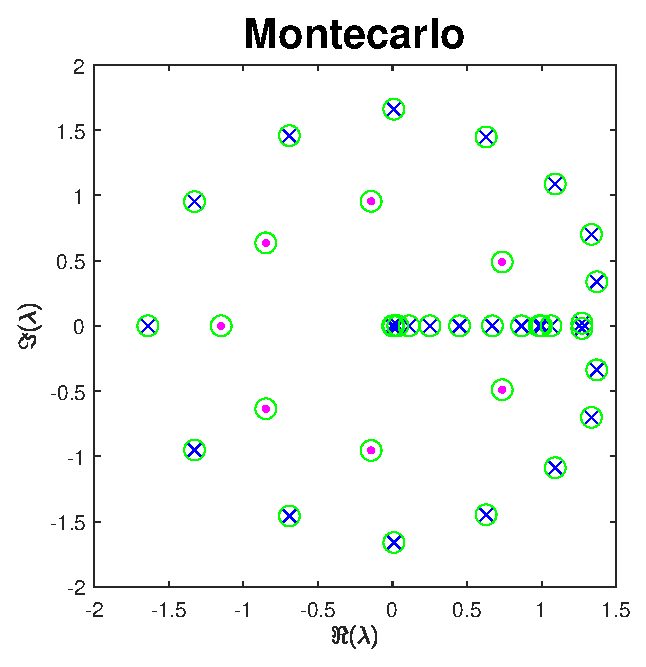
\includegraphics[width=0.25\linewidth]{../code/figures/gauss_map/ResDMD_Montecarlo.eps}
    \hspace*{\fill}
    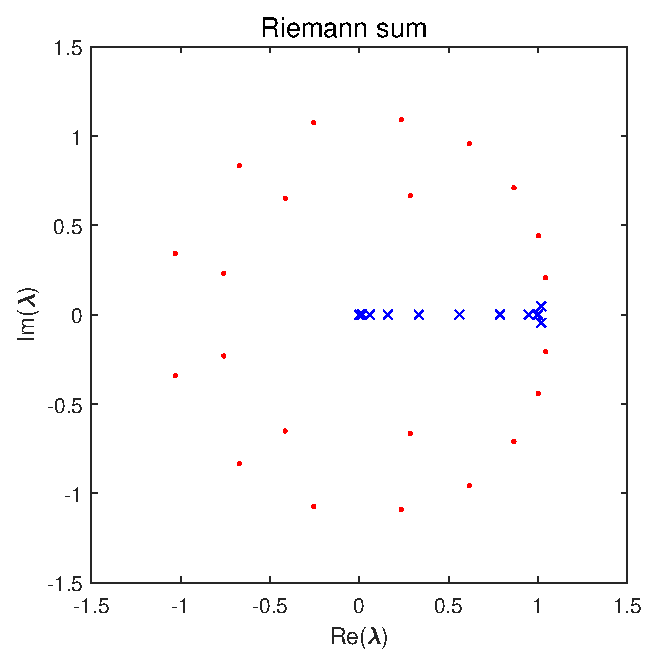
\includegraphics[width=0.25\linewidth]{../code/figures/gauss_map/ResDMD_Riemann.eps}
    \hspace*{\fill}
    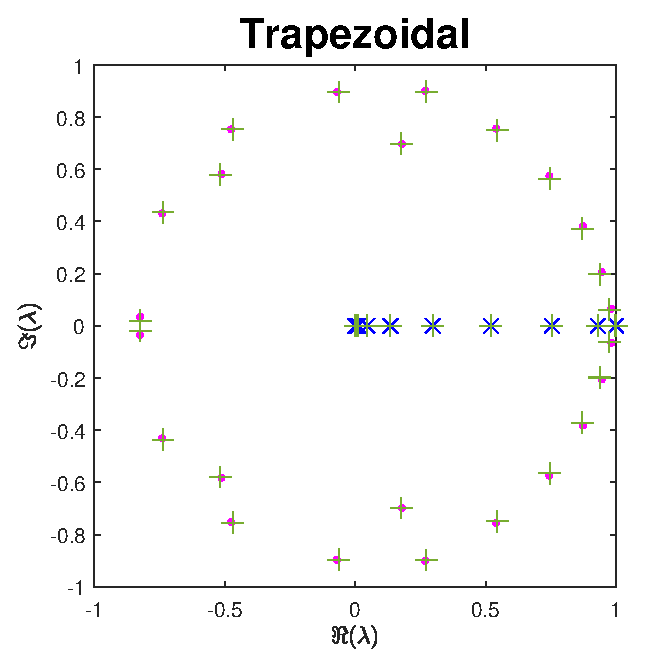
\includegraphics[width=0.25\linewidth]{../code/figures/gauss_map/ResDMD_Trapezoidal.eps}
    \hspace*{\fill}
    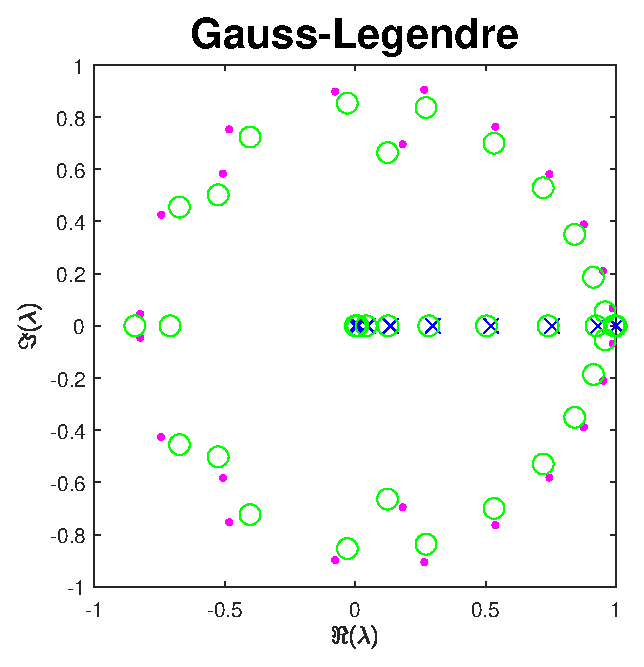
\includegraphics[width=0.25\linewidth]{../code/figures/gauss_map/ResDMD_Gauss-Legendre.eps}
    \hspace*{\fill}
}
\caption{Approximations of the eigenvalues of the Koopman Operator associated with the Gauss iterated map computed with the DMD algorithm (green pluses) and the EDMD algorithm (magenta dots and blue crosses), using different quadrature rules. The approximate eigenvalues are computed using $K=40$ observables and the blue crosses indicate the eigenvalues retained by ResDMD, with tolerance $\varepsilon = 0.01$.}
\label{fig_resdmd_quadrature_comparison}
\end{figure}

\begin{figure}[h]
\makebox[\textwidth][c]{
    \begin{subfigure}{0.45\textwidth}
        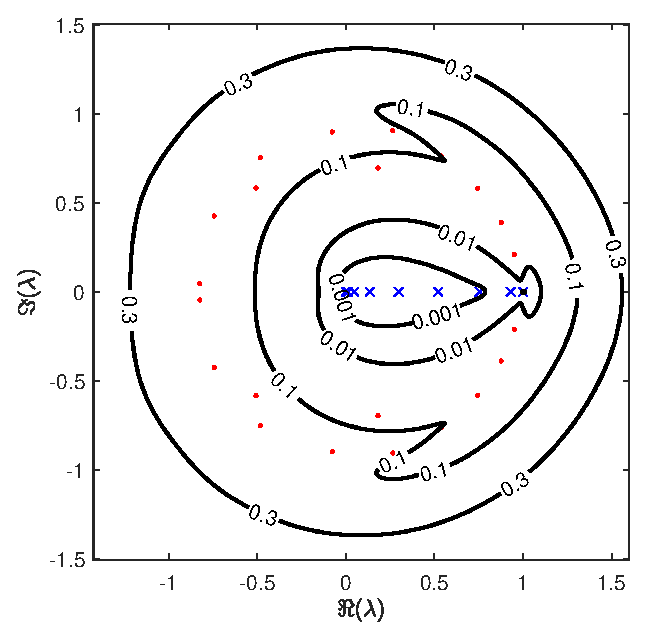
\includegraphics[width=\linewidth]{../code/figures/gauss_map/pseudospectra_contour.eps}
        \caption{Pseudospectral contours}
        \label{gauss_contours}
    \end{subfigure}\hspace*{\fill}
    \begin{subfigure}{0.45\textwidth}
        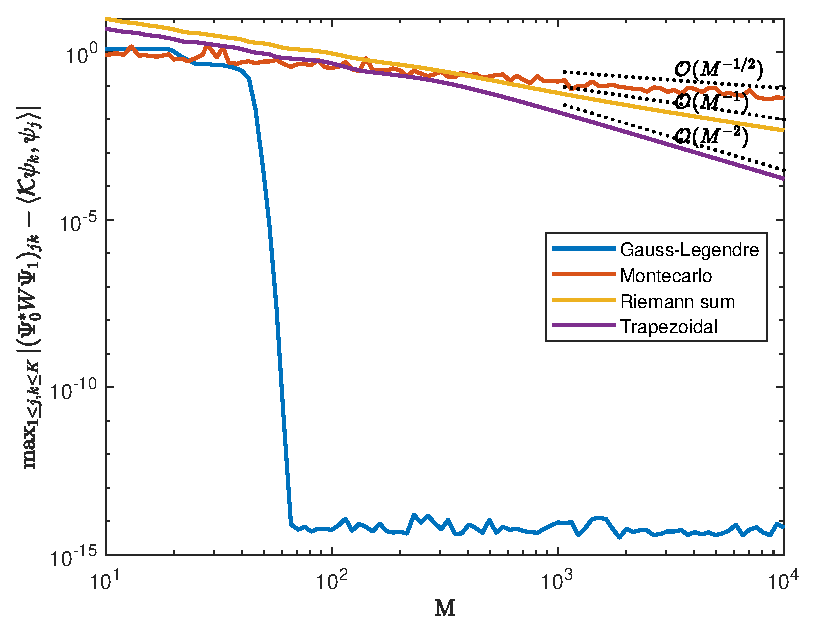
\includegraphics[width=\linewidth]{../code/figures/gauss_map/Galerkin_convergence.eps}
        \caption{Convergence of the quadrature rules}
        \label{gauss_convergence}
    \end{subfigure}\hspace*{\fill}
    }
    \caption{Contour lines of the $\varepsilon$-pseudospectrum for $\varepsilon = 0.3,\,0.1,\,0.01,\,0.001$ computed using \Cref{alg_pseudospectrum} with dictionary of $K=40$ observables (\Cref{gauss_contours}) and convergence of one of the approximate integrals for the different quadrature rules measured as $\max_{1\leq j,k \leq K} \abs{(\Psi_0^* W \Psi_1)_{jk} - \langle\mathcal{K}\psi_k, \psi_j\rangle}$ (\Cref{gauss_convergence}).}
    \label{gauss_pseudospectrum_convergence}
\end{figure}

\subsection{Nonlinear pendulum}
Let us consider the continous-time dynamical system of the nonlinear pendulum. The state variable is $\vb{x} = (x_1, x_2) = (\theta, \dot{\theta}) \in \Omega = [-\pi, \pi]_{\text{per}} \times \R$ and the differential equation governing the motion is
\begin{equation}
    \label{pendulum_equation}
    \dot{\vb{x}} = 
    \begin{bmatrix}
    \dot{x}_1 \\
    \dot{x}_2
    \end{bmatrix} = 
    \begin{bmatrix}
    x_2 \\
    -\sin(x_1)
    \end{bmatrix}.
\end{equation}
We consider the corresponding discrete-time dynamical system with time-step $\Delta_t = 0.5.$ and the associated Koopman Operator. The system is Hamiltonian and hence the Koopman Operator is unitary \cite{koopman_hamiltonian_1931}.

The choice of the dictionary of observables is now more complex, because the function governing the motion is vector-valued (with two components) and periodic in the first component. Since the motion is periodic in $x_1\in[-\pi,\pi]_{\text{per}}$, it is natural to use the Fourier basis $\{e_n\}_{n\in\mathbb{Z}}$ in $x_1$ to describe the motion in this direction. Similarly, to approximate the motion in the direction of $x_2$ one might decide to use the Hermite functions $\{h_n\}_{n\in\mathbb{N}}$, which form a basis of the Hilbert space $L^2(\R)$. Therefore, we would ideally consider observables of the form $\phi(x_1, x_2) = \sum_{n\in\mathbb{Z},\,m\in\mathbb{N}} \alpha_{n,m} e_n(x_1)\cdot h_m(x_2)$ for some coefficients $\{\alpha_{n,m}\}\in\C$. However, our dictionary of observables must be finite and we need to decide a criterion to truncate the sum. Observe that there isn't a natural ordering as if the indices were in $\mathbb{N}$ or $\mathbb{Z}$. Since we want to be able to approximate the (components of the) full state observable, it is important to have the indices $\{(n,0)\}_{n=0}^{n_{\max}}$ and $\{(0,m)\}_{m=-m_{\max}}^{m_{\max}}$ with $n_{\max},\,m_{\max}$ as high as possible. Selecting the indices in the rectangle $\{(n,m)\,:\,-n_{\max}\leq n\leq n_{\max},\,\, 0\leq m\leq m_{\max}\}$ would make the size of the dictionary grow too fast in $n_{\max}$ and $m_{\max}$, thus we use an hyperbolic cross approximation \cite{dung_hyperbolic_2017}, i.e. we select the indices in the hyperbolic cross $\{(n,m)\,:\, \max(n,1)\cdot \max(m,1)\leq N \}$, where $N$ is called the order of the hyperbolic cross approximation.

Using \Cref{alg_pseudospectrum} we compute an approximation of the $\varepsilon$-pseudospectrum for $\varepsilon = 0.25$, first using $K=193$ observables and $M = 10^4$ data points, then employing $K=1265$ and $M = 9 \times 10^4$. As the size $K$ of the dictionary increases, the approximation of the $\varepsilon$-pseudospectrum approaches the annulus with internal radius 0.75 and external radius 1.25(see \Cref{pendulum_pseudospectrum}). We also compute approximation of the eigenfunctions associated with the eigenvalues $\lambda = \exp(0.4932 i), \,\lambda = \exp(0.9765 i), \,\lambda = \exp(1.4452 i), \,\lambda = \exp(1.8951 i), \,$ (see \Cref{pendulum_phase_portraits}).

\begin{figure}[h]
\makebox[\textwidth][c]{
    \begin{subfigure}{0.45\textwidth}
        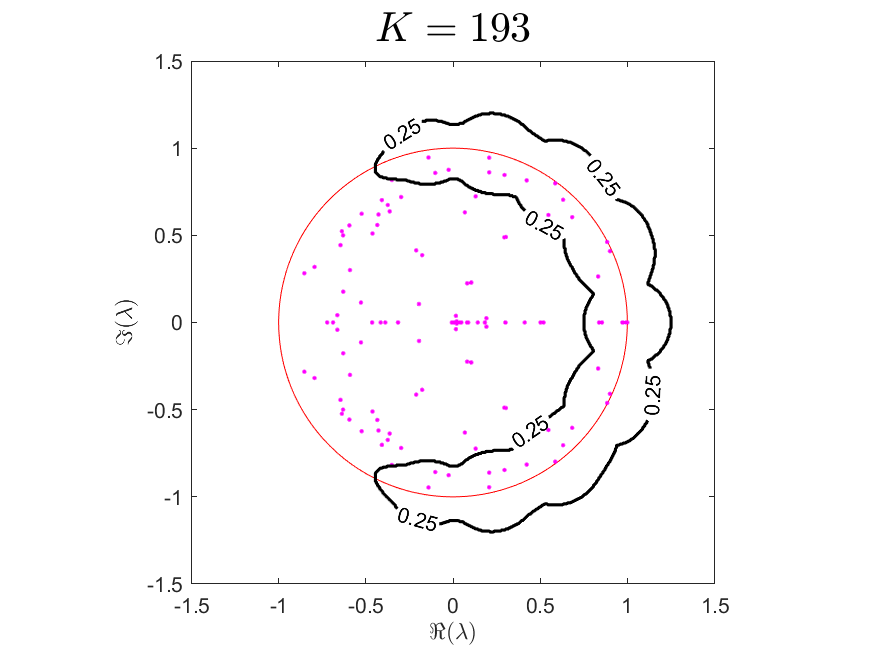
\includegraphics[width=\linewidth]{../code/figures/pendulum/pendulum_N193.png}
    \end{subfigure}\hspace*{\fill}
    \begin{subfigure}{0.45\textwidth}
        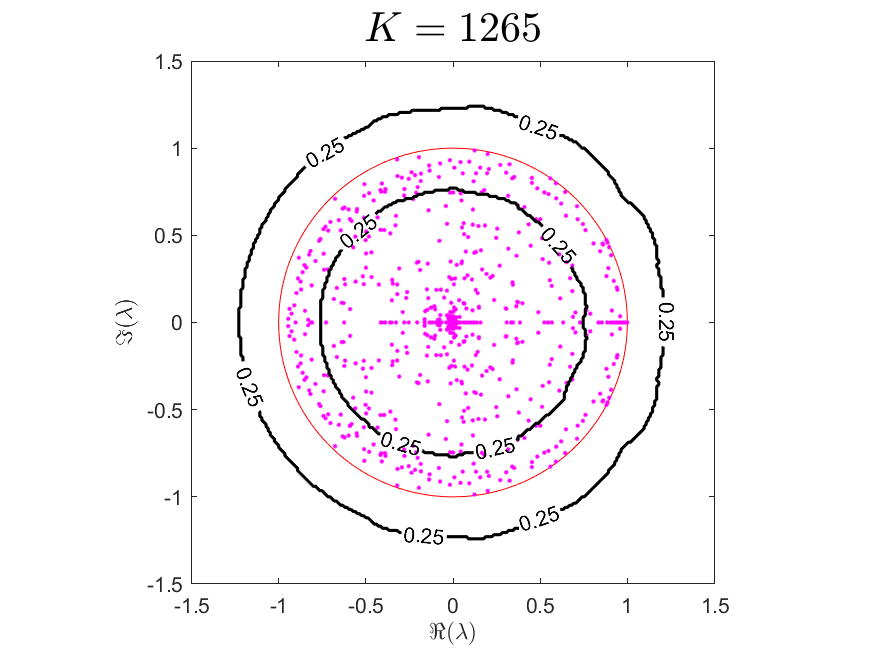
\includegraphics[width=\linewidth]{../code/figures/pendulum/pendulum_N1265.png}
    \end{subfigure}\hspace*{\fill}
        }
    \caption{Contour lines of the $\varepsilon$-pseudospectrum for $\varepsilon = 0.25$ computed using \Cref{alg_pseudospectrum} with hyperbolic cross approximation. On the left the approximation obtained using a dictionary of $K=193$ observables and $M = 10^4$ data points, on the right the one obtained with $K=1265$ and $M = 9 \times 10^4$.}
    \label{pendulum_pseudospectrum}
\end{figure}

\begin{figure}[h]
\centering
\makebox[\textwidth][c]{
        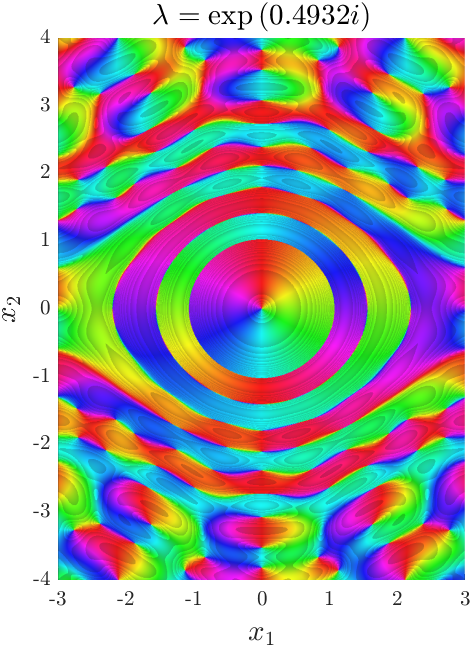
\includegraphics[width=0.25\linewidth]{../code/figures/pendulum/phase_portrait_4932.png}
        \hspace*{\fill}
        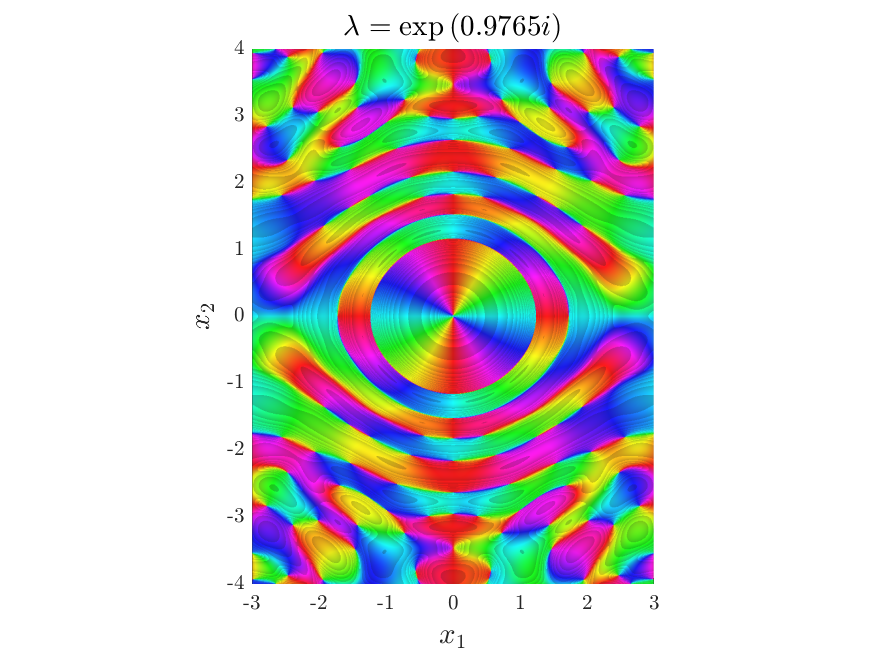
\includegraphics[width=0.25\linewidth]{../code/figures/pendulum/phase_portrait_9765.png}
        \hspace*{\fill}
        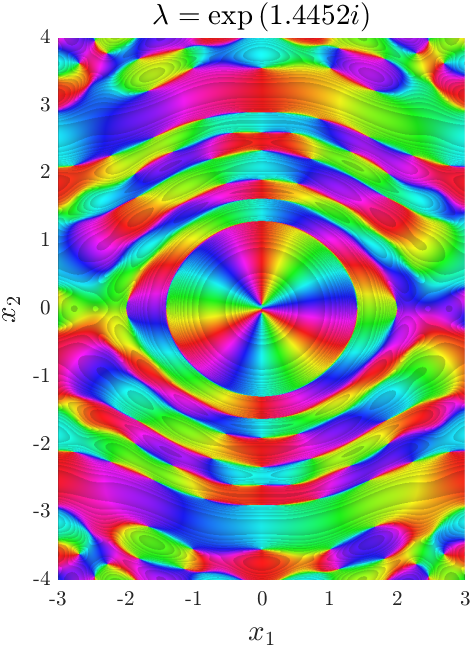
\includegraphics[width=0.25\linewidth]{../code/figures/pendulum/phase_portrait_14452.png}
        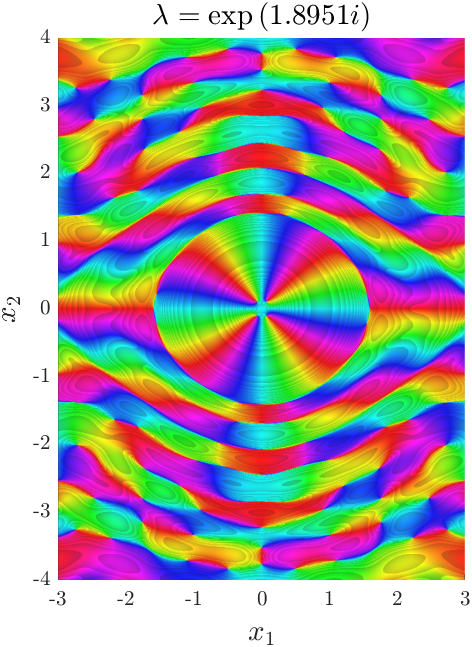
\includegraphics[width=0.25\linewidth]{../code/figures/pendulum/phase_portrait_18951.png}
        \hspace*{\fill}}
        \caption{Phase portraits of the approximate eigenfunctions of the nonlinear pendulum, where the color illustrates the complex argument of the eigenfunction. Lines of constant modulus are plotted as shadowed steps.}
        \label{pendulum_phase_portraits}
\end{figure}

\section{A kernel-based approach for high dimensional data}
Until now, we supposed that the number of snapshots was large compared to the size of the dictionary, which also controls the number of eigenpairs approximated. However, when dealing with high dimensional data, we are usually in the opposite regime, where $K \gg M$. Indeed, as the dimension of the state space increases, the number of functions needed to have a rich enough dictionary overgrows. This blowup of the size $K$ of the dictionary occurs frequently in data-driven and Machine Learning related applications \cite{budisic_applied_2012, rowley_spectral_2009, schmid_dynamic_2010}, and it can be regarded as a facet of the so-called \emph{curse of dimensionality} \cite{bishop_pattern_2006}. 

\subsection{Kernelized EDMD (K-EDMD)}
The EDMD algorithm necessitates the computation of the matrices $(\Psi_0^*\vb*{W}\Psi_0)$ and $(\Psi_0^*\vb*{W}\Psi_1)$, which requires $\mathcal{O}(MK^2)$ flops, and solving an eigenvalue problem associated to the matrix $\vb*{K}\in\C^{K\times K}$, which costs $\mathcal{O}(K^3)$ flops. For large values of $K$, such computations are impractical. \emph{Kernelized EDMD} (K-EDMD) \cite{williams_kernel-based_2015} uses the kernel trick \cite{bishop_pattern_2006} to efficiently compute a matrix $\hat{\vb*{K}}\in\C^{M\times M}$ that has the same non-zero eigenvalues as $\vb*{K}$. The computation of such a matrix relies on the following proposition.

\begin{prop}[\cite{colbrook_rigorous_2021}]
Let $\sqrt{\vb*{W}}\Psi_0 = \vb*{Q}\vb*{\Sigma}\vb*{Z}^*$ be a SVD, where $\vb*{\Sigma}\in\C^{M\times M}$ and let us define
\begin{equation}
    \label{kedmd_matrix}
    \hat{\vb*{K}} = (\vb*{\Sigma}^{\dagger}\vb*{Q}^*)(\sqrt{\vb*{W}}\Psi_1\Psi_0\sqrt{\vb*{W}})(\vb*{Q}\Sigma^{\dagger})\in\C^{M \times M}.
\end{equation}
Then $(\lambda,\,\vb{v})$ with $\lambda\neq 0$ is an eigenpair of $\hat{\vb*{K}}$ if and only if $(\lambda,\,\vb*{Z}\vb{v})$ is an eigenpair of $\vb*{K}$, where $\vb*{K}$ is defined in \eqref{discretized_problem_solution}.
\end{prop}
\begin{proof}
Let us recall that the matrix $\vb*{K}$ is defined in \eqref{discretized_problem_solution} as $\vb*{K} = (\Psi_0^*\vb*{W}\Psi_0)^{\dagger}(\Psi_0^*\vb*{W}\Psi_1)$. For a generic matrix $\vb*{A}$, the following two properties of the Moore-Penrose inverse hold: $(\vb*{A}^*\vb*{A})^{\dagger}\vb*{A}^* = \vb*{A}^{\dagger}$ and $\range(\vb*{A}^{\dagger}) = \range(\vb*{A}^*)$, where $\range(\vb*{A})$ denotes the Span of the columns (or range) of $\vb*{A}$. Applying these two properties to the matrix $\vb*{A} = \sqrt{\vb*{W}}\Psi_0$ it follows: 
\begin{equation*}
    \begin{split}
        &\vb*{K} = (\Psi_0^*\vb*{W}\Psi_0)^{\dagger}(\Psi_0^*\vb*{W}\Psi_1) = (\sqrt{\vb*{W}}\Psi_0)^{\dagger} \sqrt{\vb*{W}}\Psi_1 \\
        &\range(\vb*{K}) \subseteq \range((\sqrt{\vb*{W}}\Psi_0)^{\dagger}) = \range(\sqrt{\vb*{W}}\Psi_0)^*)
    \end{split}
\end{equation*}
Hence any eigenvector $\vb{v}$ such that $\vb*{K}\vb{v} = \lambda \vb{v}$ with $\lambda \neq 0$ can be written as $\vb{v} = (\sqrt{\vb*{W}}\Psi_0)^*\tilde{\vb{v}} = \vb*{Z}\vb*{\Sigma}\vb*{Q}^*\tilde{\vb{v}} = \vb*{Z}\hat{\vb{v}}$ for some $\hat{\vb{v}}$. Thus:
\begin{equation*}
    \lambda \vb*{Z}\hat{\vb{v}} = \vb*{K}\vb*{Z}\hat{\vb{v}} = (\sqrt{\vb*{W}}\Psi_0)^{\dagger} \sqrt{\vb*{W}}\Psi_1 \vb*{Z}\hat{\vb{v}} = \vb*{Z}\left[(\vb*{\Sigma}^{\dagger}\vb*{Q}^*)(\sqrt{\vb*{W}}\Psi_1\Psi_0\sqrt{\vb*{W}})(\vb*{Q}\Sigma^{\dagger})\right] \hat{\vb{v}}
\end{equation*}
and multiplying by $\vb*{Z}^*$ on the right we obtain that if $(\lambda,\,\vb{v})$ is an eigenpair of $\vb*{K}$ with $\lambda\neq 0$, then $(\lambda,\,\hat{\vb{v}} = \vb*{Z}^*\vb{v})$ is an eigenpair of $\hat{\vb*{K}}$. 

Vice versa, if $(\lambda,\,\vb{v})$ is an eigenpair of $\hat{\vb*{K}}$, then:
\begin{equation*}
    \vb*{K}\vb*{Z}\vb{v} = \vb*{Z}\hat{\vb*{K}}\vb{v} = \lambda\vb*{Z}\vb{v}
\end{equation*}
i.e. $(\lambda,\,\vb*{Z}\vb{v})$ is an eigenpair of $\vb*{K}$.
\end{proof}

Now observe that to build the matrix $\hat{\vb*{K}}$ we just need to compute inner products of evaluation of our dictionary. The matrices $\vb*{Q}$ and $\vb*{\Sigma}$ can be obtained from the eigenvalue decomposition of $\sqrt{\vb*{W}}\Psi_0\Psi_0^*\sqrt{\vb*{W}} = \vb*{Q}\vb*{\Sigma}^2\vb*{Q}^*$, and both $(\sqrt{\vb*{W}}\Psi_0\Psi_0^*\sqrt{\vb*{W}})$ and $(\sqrt{\vb*{W}}\Psi_1\Psi_0^*\sqrt{\vb*{W}})$ can be computed using inner products only. Indeed, recalling that $\Psi(\vb{x})$ is a row vector:
\begin{equation}
    \label{kernel_matrices}
    \begin{split}
        (\sqrt{\vb*{W}}\Psi_0\Psi_0^*\sqrt{\vb*{W}})_{ij} &= \sqrt{w_i} \Psi(\vb{x}_0^{(i)}) \Psi(\vb{x}_0^{(j)})^* \sqrt{w_j}\\
        (\sqrt{\vb*{W}}\Psi_1\Psi_0^*\sqrt{\vb*{W}})_{ij} &= \sqrt{w_i} \Psi(\vb{x}_1^{(i)}) \Psi(\vb{x}_0^{(j)})^* \sqrt{w_j}.
    \end{split}
\end{equation}
The kernel trick \cite{bishop_pattern_2006} is a common technique used to compute these inner products implicitly. Instead of first evaluating the dictionary $\Psi(\vb{x})$ and then computing the inner product, that would require $\mathcal{O}(K)$ operations, we compute $\kappa(\vb{x}, \vb{y}) = \Psi(\vb{x})\Psi(\vb{y})^*$ for a suitably defined kernel $\kappa$. It is crucial that the kernel $\kappa$ does not compute the inner product directly, but it does so implicitly in $\mathcal{O}(d)$ operations. Thus the matrices $(\sqrt{\vb*{W}}\Psi_0\Psi_0^*\sqrt{\vb*{W}})$ and $(\sqrt{\vb*{W}}\Psi_1\Psi_0^*\sqrt{\vb*{W}})$ can be calculated in $\mathcal{O}(dM^2)$ operations, without suffering from the large size of the dictionary. The total complexity of computing $\hat{\vb*{K}}$ and solving the associated eigenvalue problem is $\mathcal{O}(d M^2 + M^3)$, significantly lower than the $\mathcal{O}(M K^2+K^3)$ cost of applying EDMD directly. 

\subsubsection{Computing the Koopman eigenvalues, eigenfunctions and modes}
Once we have computed the matrix $\hat{\vb*{K}}$ and its eigendecomposition, we still need to understand how to retrieve from it an approximation of the Koopman eigenvalues, eigenfunctions and modes. The eigenvalues of $\hat{\vb*{K}}$ can be directly used as approximation of the Koopman eigenvalues. Let $\hat{\bm{\Xi}} = \left[\hat{\bm{\xi}}_1,\dots,\hat{\bm{\xi}}_M\right]$ be the matrix of the eigenvectors of $\hat{\vb*{K}}$, the vector of approximate Koopman eigenfunctions $\Phi(\vb{x}) = \left[\phi_1(\vb{x}), \dots, \phi_M(\vb{x})\right]$ can be written as $\Phi = \Psi\vb*{Z}\hat{\bm{\Xi}} = \Psi (\Psi_0^*\sqrt{\vb*{W}})(\vb*{Q}\Sigma^{\dagger}) \hat{\bm{\Xi}}$. All we have done so far would not be useful if suffered from the size of the dictionary when approximating the Koopman eigenfunctions. Fortunately, it is possible to express them using kernels only. Indeed:
\begin{equation}
    \label{kernel_eigenfunctions}
    \begin{split}
        \phi_k(\vb{x}) &= \Psi(\vb{x}) (\Psi_0^*\sqrt{\vb*{W}})(\vb*{Q}\Sigma^{\dagger}) \hat{\bm{\xi}}_k =\\
        &= \left[\sqrt{w_1} \kappa(\vb{x}, \vb{x}_0^{(1)}), \dots, \sqrt{w_M} \kappa(\vb{x}, \vb{x}_0^{(M)})\right](\vb*{Q}\Sigma^{\dagger}) \hat{\bm{\xi}}_k
    \end{split}
\end{equation}
so that the size $K$ of the dictionary does not enter any of the computations.

To compute the Koopman modes of the full state observable, we consider equation \eqref{koopman_modes} and we evaluate it at each of the data points using the approximate eigenfunctions we just obtained. When evaluated at $\vb{x}_0^{(i)}$ the equation reads:
\begin{equation}
    \label{kedmd_modes_pointwise}
    \vb{x}_0^{(i)} = \sum_{j = 1}^M \phi_j(\vb{x}_0^{(i)})\hat{\vb{v}}_{j} + \vb{r}_i
\end{equation}
where $\{\hat{\vb{v}}_{j}\}_{j=1}^M$ are the Koopman modes that we want to retrieve and $\vb{r}_i$ is a residual that must be minimized. If we introduce the matrices
\begin{equation}
    \begin{split}
    \vb*{X} = 
    \begin{bmatrix}
    (\vb{x}_0^{(1)})^T \\
    \vdots \\
    (\vb{x}_0^{(M)})^T
    \end{bmatrix}&,
    \\ 
    \Phi_0 = 
    \begin{bmatrix}
    \Phi(\vb{x}_0^{(1)}) \\
    \vdots \\
    \Phi(\vb{x}_0^{(M)})
    \end{bmatrix}&
    = \Psi_0 \vb*{Z}\hat{\bm{\Xi}} = \Psi_0 (\Psi_0^*\sqrt{\vb*{W}})(\vb*{Q}\Sigma^{\dagger}) \hat{\bm{\Xi}} =\\
    & = \sqrt{\vb*{W}^{-1}} \vb*{Q}\vb*{\Sigma}^2\vb*{Q}^*\vb*{Q}\Sigma^{\dagger}\hat{\bm{\Xi}} = \sqrt{\vb*{W}^{-1}} \vb*{Q}\Sigma\hat{\bm{\Xi}}
    \end{split}
\end{equation}
i.e. the data-points matrix and the matrix of the eigenfunctions values at those points, \eqref{kedmd_modes_pointwise} can be rewritten as
\begin{equation}
    \label{kedmd_modes_matrix}
    \vb*{X} = \Psi_0 \hat{\vb*{V}} + \vb*{R}.
\end{equation}
The solution to the least squares problem is 
\begin{equation}
    \hat{\vb*{V}} =  
    \begin{bmatrix}
    \hat{\vb{v}}_1^T \\
    \vdots \\
    \hat{\vb{v}}_M^T
    \end{bmatrix}
    = \Psi_0^{\dagger} \vb*{X} = \hat{\bm{\Xi}}^{-1} \Sigma^{\dagger} \vb*{Q}^* \sqrt{\vb*{W}} \vb*{X}.
\end{equation}
Hence the approximation of the $j$-th Koopman mode is 
\begin{equation}
    \label{kedmd_modes}
    \hat{\vb{v}}_j = (\hat{\vb{u}}_j^* \Sigma^{\dagger} \vb*{Q}^* \sqrt{\vb*{W}} \vb*{X})^T
\end{equation}
where $\hat{\vb{u}}_j$ is a left eigenvector of $\hat{\vb*{K}}$ appropriately scaled so that $\hat{\vb{u}}_j^*\hat{\bm{\xi}}_i = \delta_{ij}$.

\subsubsection{The choice of the kernel}
Even if in the previous discussion we supposed that, given a dictionary $\Psi(\vb{x})$, there exists a kernel $\kappa$ that computes $\kappa(\vb{x}, \vb{y}) = \Psi(\vb{x})\Psi(\vb{y})^*$ implicitly, in effect it is usually the choice of $\kappa$ that defines the dictionary. One of the most simple kernels is the polynomial kernel $\kappa(\vb{x}, \vb{y}) = (1 + \vb{x}^*\vb{y})^{n}$, which is equivalent to a dictionary that can represent all polynomials up to degree $n$. Increasing $n$ the implicitly defined dictionary becomes larger, at the cost of a worst conditioning of the resulting matrices. For this reason, taking inspiration from Machine Learning techniques, other kernels could be considered, such as the widely used radial basis function kernel (RBF kernel), $\kappa(\vb{x}, \vb{y}) = \exp(-\norm{\vb{x}-\vb{y}}^2 / \sigma^2)$.

\begin{algorithm}[h]
\caption{\textbf{: Kernelized EDMD (K-EDMD)}}
\label{alg_kedmd}
\textbf{Input:} Snapshot pairs of the system state, $\{(\vb{x}_0^{(m)}, \vb{x}_1^{(m)})\}_{m = 1}^M$, quadrature weights $\{w_m\}_{m = 1}^M$, kernel $\kappa = \kappa(\cdot\,,\,\cdot)$.
\begin{algorithmic}[1]
\State  Compute the matrices $\hat{\vb*{G}} = \sqrt{\vb*{W}}\Psi_0\Psi_0^*\sqrt{\vb*{W}}$ and  $\hat{\vb*{A}} = \sqrt{\vb*{W}}\Psi_1\Psi_0^*\sqrt{\vb*{W}}$, exploiting that $\hat{\vb*{G}}_{ij} = \sqrt{w_i} \kappa(\vb{x}_0^{(i)},\, \vb{x}_0^{(j)}) \sqrt{w_j}$ and
$\hat{\vb*{A}}_{ij} = \sqrt{w_i} \kappa(\vb{x}_1^{(i)},\, \vb{x}_0^{(j)}) \sqrt{w_j}$.
\State Compute the eigenvalue decomposition of $\hat{\vb*{G}} = \vb*{Q}\vb*{\Sigma}^2\vb*{Q}^*$.
\State Compute $\hat{\vb*{K}} = (\vb*{\Sigma}^{\dagger}\vb*{Q}^*)\hat{\vb*{A}} (\vb*{Q}\Sigma^{\dagger})$.
\State Solve the eigenvalue problem of $\hat{\vb*{K}}\hat{\bm{\xi}} = \lambda \hat{\bm{\xi}}$.
\State Obtain the eigenfunctions as $\phi_k(\vb{x}) = \left[\sqrt{w_1} \kappa(\vb{x}, \vb{x}_0^{(1)}), \dots, \sqrt{w_M} \kappa(\vb{x}, \vb{x}_0^{(M)})\right](\vb*{Q}\Sigma^{\dagger}) \hat{\bm{\xi}}_k$.
\If{want to compute eigenmodes}
    \State Compute the left eigenvectors $\vb{u}_j$ of $\hat{\vb*{K}}$ appropriately scaled so that $\hat{\vb{u}}_j^*\hat{\bm{\xi}}_i = \delta_{ij}$.
    \State Compute $\hat{\vb*{B}} = \Sigma^{\dagger} \vb*{Q}^* \sqrt{\vb*{W}} \vb*{X}$.
    \State Obtain the modes as $\hat{\vb{v}}_j = (\hat{\vb{u}}_j^* \hat{\vb*{B}})^T$.
\EndIf
\end{algorithmic}
\textbf{Output:} Approximation of the eigenvalues ($\lambda_j$), eigenfunctions ($\phi_j$) and, eventually, eigemodes ($\vb{v}_j$).
\end{algorithm}

\subsection{Kernelized ResDMD (K-ResDMD)}
At this point, it is a natural question how one could extend ResDMD with a kernelized approach. Unfortunately, applying \Cref{alg_resdmd} with K-EDMD instead of EDMD makes the approximate residual always vanish (see \cite{colbrook_rigorous_2021}, Proposition 6.2). Basically, since the size of our function space is larger than the number of snapshots, we can "interpolate", and we are actually overfitting our dataset. Similarly to what is done when training and testing a Machine Learning model, to have a reliable estimate of the residual for approximate eigenpairs, we need to compute it using quadrature points that have not been used at the "interpolation stage" and that, at least ideally, are independent of the ones previously employed. This idea leads to the following multi-step approach:
\begin{enumerate}
    \item Split the snapshot data into two (ideally independent) sets $\{(\vb{x}_0^{(j)},\,\vb{x}_1^{(j)})\}_{j=1}^{M'}$ and  $\{(\vb{y}_0^{(j)},\,\vb{y}_1^{(j)})\}_{j=1}^{M''}$, with $M'' \geq M'$.
    \item Apply K-EDMD to the first data set $\{(\vb{x}_0^{(j)},\,\vb{x}_1^{(j)})\}_{j=1}^{M'}$, and compute a dictionary that Spans the function space generate by the approximations of dominant $K' < M'$ eigenfunctions (see \Cref{alg_kresdmd} for the details). Let us denote this dictionary as $\Psi(x) = \left[\psi_1(\vb{x}), \dots, \psi_{K'}(\vb{x})\right]$.
    \item Apply \Cref{alg_resdmd} or \Cref{alg_pseudospectrum} with snapshot data $\{(\vb{y}_0^{(j)},\,\vb{y}_1^{(j)})\}_{j=1}^{M''}$ and dictionary $\Psi(x)$.
\end{enumerate}
As summarized in \Cref{alg_kresdmd} in the first stage, we reduce the size of the dictionary implicitly defined by the kernel to $K'$, hoping to obtain a good dictionary that already captures the essential dynamics. Then this dictionary is used as a basis for the ResDMD algorithm, which computes reliable approximations of the eigenpairs of the Koopman operator. This also provides an a posteriori check of the quality of the dictionary obtained in the first stage.

\begin{algorithm}[h]
\caption{\textbf{: Kernelized ResDMD (K-ResDMD)}}
\label{alg_kresdmd}
\textbf{Input:} Snapshot pairs of the system state, $\{(\vb{x}_0^{(m)}, \vb{x}_1^{(m)})\}_{m = 1}^M$, quadrature weights $\{w_m\}_{m = 1}^M$, kernel $\kappa = \kappa(\cdot\,,\,\cdot)$, hyperparameters $M', \,M'', \,K'$.
\begin{algorithmic}[1]
\State  Split the snapshot data into $\{(\vb{x}_0^{(j)},\,\vb{x}_1^{(j)})\}_{j=1}^{M'}$ and  $\{(\vb{y}_0^{(j)},\,\vb{y}_1^{(j)})\}_{j=1}^{M''}$, with $M = M' + M''$ and $M'' \geq M' > K'$.
\State Apply K-EDMD (\Cref{alg_kedmd}) with snapshot pairs $\{(\vb{x}_0^{(j)},\,\vb{x}_1^{(j)})\}_{j=1}^{M'}$: compute the dominant $K' < M'$ eigenvectors of $\hat{\vb*{K}}$ and stack them into $\hat{\bm{\Xi}} = \left[\hat{\bm{\xi}}_1, \dots, \hat{\bm{\xi}}_{K'}\right]$. 
\State Orthogonalize the colums of $\hat{\bm{\Xi}}$ to $\vb*{P} = [\vb{p}_1, \dots, \vb{p}_{K'}]$.
\State Apply \Cref{alg_resdmd} or \Cref{alg_pseudospectrum} with snapshot data $\{(\vb{y}_0^{(j)},\,\vb{y}_1^{(j)})\}_{j=1}^{M''}$ and dictionary $\{\psi_j\}_{j = 1}^{K'}$ defined by
\begin{equation*}
    \psi_j(\vb{x}) = \left[\sqrt{w_1} \kappa(\vb{x}, \vb{x}_0^{(1)}), \dots, \sqrt{w_M} \kappa(\vb{x}, \vb{x}_0^{(M')})\right](\vb*{Q}\Sigma^{\dagger})\, \vb{p}_j
\end{equation*}
\end{algorithmic}
\textbf{Output:} According to the algorithm chosen in the final step.
\end{algorithm}
